% !TeX root = ../dissertation.tex

\section{Rare events and asymptotic analysis}
\footnotetextonly{\Cref{sec:LDP_constant,sec:LDP_random} previously appeared in the following open-access article: \fullcite{KuoShresthaSinhaSundar2022}.}

In mathematics, particularly in analysis, we are frequently concerned with asymptotic behavior of mathematical objects. Elementary probability theory gives us some simple tools to know the asymptotic behavior of means of random variables. First, the law of large numbers says that if we repeat the same experiment a large number of times, we should expect the empirical mean of the result to be close to the theoretical mean.

To formalize this, assume we have a sequence of independent and identically distributed (i.i.d.) integrable random variables \( \br{X_n}_{n = 1}^∞ \) with such that \( \E\br{X_1} = m \). Let \( S_n = ∑_{i = 1}^n X_i \) be the sum and \( \overline{X}_n = \frac{S_n}{n} \) be the empirical mean of \( n \) such random variables.
\begin{theorem}  \index{law of large numbers}
    \begin{align*}
        \overline{X}_n → m \text{ as } n → ∞  \quad  \text{almost surely or in \( \Pr \).}
    \end{align*}
    This is called the \emph{strong law of large numbers} if the convergence is almost surely. If the convergence is in probability, then the theorem is called the \emph{weak law of large numbers}.
\end{theorem}
Since almost sure convergence implies convergence in probability, the strong law implies the weak law. Even though it is called a \textquote{law} for historical reasons, it is a theorem of probability theory. Using notation from asymptotic analysis, we can write this as \( \overline{X}_n = m + o(1) \).

The law of large numbers do not give us any knowledge of how far down the sequence we have to go in order for our empirical means to come \textquote{close} to the theoretical mean. The central limit theorem helps in this regard.

\begin{theorem}[Lindeberg–Lévy]  \index{central limit theorem!Lindeberg–Lévy}
    Assume the setting above along with the condition that \( \V\br{X_1} = σ^2 < ∞ \). Let \( Z ∼ N(0, 1) \) be a standard normal variable. Then
    \begin{equation*}
        \sqrt{n} \br{\overline{X}_n - m} → σ Z  \quad  \text{in distribution.}
    \end{equation*}
    Alternatively, in terms of the empirical sum \( S_n \), we can write this as
    \begin{equation*}
        \frac{S_n - n m}{\sqrt{n}} → σ Z  \quad  \text{in distribution.}
    \end{equation*}
\end{theorem}

Therefore, the central limit theorem gives us one more level of detail. Asymptotically, it says that
\begin{equation*}
    \overline{X}_n ≃ m + \frac{1}{\sqrt{n}} σ Z + o\br{\frac{1}{\sqrt{n}}} .
\end{equation*}
The tradeoff here is that we now have to contend ourselves with the weaker sense of convergence is in distribution.

Can we do better? Let us look at a specific example. Suppose that now all our random variables are i.i.d. standard normal, that is \( X_1 ∼ N(0, 1) \). Then the moment generating function of \( X_1 \) is given by \( M(θ) = \E\br{e^{θ X_1}} = e^{\frac12 θ^2} \). We write the moment generating function of \( S_n \) as
\begin{equation*}
    M_{S_n}(θ)
    =  \E\br{e^{θ S_n}}
    =  \E\br{e^{θ ∑_{i = 1}^n X_i}}
    =  \E\br{∏_{i = 1}^n e^{θ X_i}}
    =  ∏_{i = 1}^n \E\br{e^{θ X_i}} ,
\end{equation*}
where we used the independence assumption in the last step. Using the identical distribution assumption, we get
\begin{equation*}
    M_{S_n}(θ)
    =  \br{\E\br{e^{θ X_1}}}^n
    =  \br{e^{\frac12 θ^2}}^n
    =  e^{\frac12 θ^2 n}
    =  e^{o(n)} .
\end{equation*}
On the other hand, using law of large numbers, we get \( S_n = n \overline{X}_n = o(n) \), and so
\begin{equation*}
    M_{S_n}(θ)
    =  \E\br{e^{θ S_n}}
    =  \E\br{e^{o(n)}} ,
\end{equation*}
which does not equal \( e^{o(n)} \) that we obtained using the moment generating function approach.

Why does the moment generating function give us better results than the law of large numbers? For one, the moment generating function actually takes into account the distribution of the random variables and does not use any approximation. However, there is another simple explanation for this. When we compute the expectations of random variable that can take very large values with very small probabilities, we cannot simply ignore the contributions of such values. This is because the product \( p q \), where \( p \) is large and \( q \) is small depends on the magnitude of \( p \) and \( q \), and can be quite large.

These kinds of problems are the mainstay of the insurance industry. Actuaries have to compute the expectation of net payout given that probabilities of accidents are quite small. Consider the following real-world problem. Let the i.i.d. random variables \( X_n \) denote the value of claims received by an insurance company on the \( n \)th month. The steady income for the company per month is the premium \( x \). The company wants to use a planning period of \( n \) months to set the value of \( x \) so that they make a profit on average with a certain degree of certainty. Essentially, the goal is to determine \( x \) such that \( \Pr\br{\overline{X}_n ≥ x} < ϵ \), where \( ϵ \) is an acceptable error probability. Therefore, it is hardly surprising that the theory of large deviations was started by actuarial mathematicians, prime among them being the Swedish mathematician Harald Cramér. However, it was Varadhan\cite{Varadhan1966} who formally defined large deviations and unified the various results into a coherent theory, for which he was awarded the Abel Prize in 2007.

To get an idea of what Cramér showed, we use Markov's inequality\index{Markov's inequality} to obtain exponential tail bounds of \( \overline{X}_n \). Suppose \( X_1 \) has a finite moment generating function \( M \). For an arbitrary \( θ > 0 \), using the i.i.d. nature of \( \br{X_n} \), we get
\begin{align*}
    \Pr\bc{\overline{X}_n ≥ x}
    & =  \Pr\bc{e^{θ n \overline{X}_n} ≥ e^{θ n x}}  \\
    & ≤  e^{-θ n x} \E\br{e^{θ n \overline{X}_n}}  \\
    & =  e^{-θ n x} M_{\overline{X}_n}(θ n)  \\
    & =  \br{e^{-θ x}}^n M(θ)^n  \\
    & =  e^{-n \br{θ x - \log M(θ)}} .
\end{align*}
Since \( θ > 0 \) is arbitrary, we have
\begin{equation*}
    \Pr\bc{\overline{X}_n ≥ x}
    ≤  \inf_θ e^{-n \br{θ x - \log M(θ)}}
    =  e^{-n \sup_θ \br{θ x - \log M(θ)}} .
\end{equation*}
Letting \( Λ^*(x) := \sup_{θ > 0} \bc{θ x - \log M(θ)} \), moving all terms dependent on \( n \) to the left, and taking \( \varlimsup \), we get
\[ \varlimsup_{n → ∞} \frac1n \log \Pr\bc{\overline{X}_n ≥ x} ≤ Λ^*(x) . \]
Now, instead of the set \( [x, ∞) \), if we consider an arbitrary closed set \( F \), we can expect
\[ \varlimsup_{n → ∞} \frac1n \log \Pr\bc{\overline{X}_n ∈ F} ≤ \inf_{x ∈ F} Λ^*(x) . \]
This is called a \emph{large deviation upper bound}.

In fact, for this case, we can also obtain a \emph{large deviation lower bound}. This means that for any arbitrary open set \( G \), we can expect
\[ \varliminf_{n → ∞} \frac1n \log \Pr\bc{\overline{X}_n ∈ G} ≥ \inf_{x ∈ G} Λ^*(x) . \]

This is the statement of the famous Cramér's theorem\index{Cramér's theorem}.
\begin{theorem}[\cite{Cramér1938}]
    The following hold.
    \begin{enumerate}
        \item  (upper bound)  For every closed set \( F \),
            \[ \varlimsup_{n → ∞} \frac1n \log \Pr\bc{\overline{X}_n ∈ F}  ≤  - \inf_{x ∈ F} Λ^*(x) . \]
        \item  (lower bound)  For every open set \( G \),
            \[ \varliminf_{n → ∞} \frac1n \log \Pr\bc{\overline{X}_n ∈ G}  ≥  - \inf_{x ∈ G} Λ^*(x) . \]
    \end{enumerate}
\end{theorem}

Putting the two bounds together, we say that \( \br{\overline{X}_n} \) follows a \emph{large deviation principle} with \emph{rate function} \( Λ^* \), and we informally write
\[ \Pr\bc{\overline{X}_n ∈ \dif x} ≍ e^{-n Λ^*(x)} . \]

In essence, the theory of large deviation allow us to find probabilities of rare events that decay exponentially.

Even though the theory of large deviations originated in the works of Scandinavian actuaries, it has become one of the central topics in probability theory, having found numerous applications in the seemingly disparate fields of dynamical systems, statistical mechanics, information theory, and fluid mechanics, among others.



\section{Large deviation principles}
We now formally define large deviation principles in a general setting. Recall that a Polish space is any space that is homeomorphic to a complete metric space having a countable dense subset.
\begin{definition}
    Let \( (𝒳, d) \) be a Polish space and \( \br{μ^ϵ}_{ϵ > 0} \) a sequence of Borel probability measures on \( 𝒳 \). Suppose \( I: 𝒳 → [0, ∞] \) is a lower semicontinuous functional. Then the sequence \( \br{μ^ϵ}_{ϵ > 0} \) is said to satisfy a \emph{large deviation principle}\index{large deviation principle} (LDP) on \( 𝒳 \) with \emph{rate function}\index{rate function} \( I \) if and only if for each Borel measurable \( E ⊆ 𝒳 \),
    \begin{equation*}
        - \inf_{x ∈ E^∘} I(x) ≤ ϵ \varliminf_{ϵ → 0} \log μ^ϵ(E) ≤ ϵ \varlimsup_{ϵ → 0} \log μ^ϵ(E) ≤ - \inf_{x ∈ \overline{E}} I(x) ,
    \end{equation*}
    where \( E^∘ \) and \( \overline{E} \) are the interior and closure of \( E \), respectively.

    Equivalently, the sequence \( \br{μ^ϵ}_{ϵ > 0} \) is said to satisfy a large deviation principle with rate function \( I \) if and only if
    \begin{enumerate}
        \item  (upper bound)\index{large deviation principle!upper bound}  for every closed set \( F ⊆ 𝒳 \),
            \[ \varlimsup_{ϵ → 0} ϵ \log μ^ϵ(F)  ≤  - \inf_{x ∈ F} I(x) , \]
        \item  (lower bound)\index{large deviation principle!lower bound}  and for every open set \( G ⊆ 𝒳 \),
            \[ \varliminf_{ϵ → 0} ϵ \log μ^ϵ(G)  ≥  - \inf_{x ∈ G} I(x) . \]
    \end{enumerate}
\end{definition}

Recall that we used the second version to write Cramér's theorem in the previous section.

The next result states how LDPs are transferred under continuous transformations.
\begin{theorem}[contraction/continuity principle {\cite[theorem 4.2.1]{DemboZeitouni1998}}]  \label{thm:LDP_continuity_principle}  \index{continuity principle}
    Let \( 𝒳 \) and \( 𝒴 \) be Hausdorff spaces and \( f: 𝒳 → 𝒴 \) a continuous function. Suppose the sequence of probability measures \( \br{μ^ϵ}_{ϵ > 0} \) on \( 𝒳 \) satisfy a large deviation principle with rate function \( I: 𝒳 → [0, ∞] \). For each \( y ∈ 𝒴 \), define \( J(y) = \inf \bc{(I ∘ \inv{f})(y)} \). Then the sequence of pushforward probability measures \( \br{μ^ϵ ∘ \inv{f}}_{ϵ > 0} \) on \( 𝒴 \) satisfy a large deviation principle with rate function \( J: 𝒴 → [0, ∞] \).
\end{theorem}

Are there situations where a large deviation principle is preserved? To answer this, we define exponential equivalence of measures.
\begin{definition}[{\cite[definition 4.2.10]{DemboZeitouni1998}}]
    Let \( (𝒳, d) \) be a Polish space with two families of measures \( \br{μ^ϵ}_{ϵ > 0} \) and \( \br{ν^ϵ}_{ϵ > 0} \) on it. Suppose there exists probability spaces \( \br{Ω, Σ_ϵ, \Pr_ϵ} \) and two families of \( 𝒳 \)-valued random variables \( \br{X^ϵ}_{ϵ > 0} \) and \( \br{Y^ϵ}_{ϵ > 0} \) with joint laws \( \br{\Pr_ϵ}_{ϵ > 0} \) and marginals \( \br{μ^ϵ}_{ϵ > 0} \) and \( \br{ν^ϵ}_{ϵ > 0} \), respectively. Moreover, for all \( δ > 0 \), the set \( \bc{ω \given (X^ϵ, Y^ϵ) ∈ E_δ} \) is \( Σ_ϵ \)-measurable, and \( \varlimsup_{ϵ → 0} ϵ \log \Pr_ϵ\br{E_δ} = -∞ \), where \( E_δ = \bc{(x, y) \given d(x, y) > δ} ⊆ 𝒳^2 \). Then the families \( \br{μ^ϵ}_{ϵ > 0} \) and \( \br{ν^ϵ}_{ϵ > 0} \) (and correspondingly \( \br{X^ϵ}_{ϵ > 0} \) and \( \br{Y^ϵ}_{ϵ > 0} \)) are called \emph{exponentially equivalent}\index{exponential equivalence}.
\end{definition}

Exponentially equivalent families of measures induce the same large deviation principle. This is the content of the following theorem.
\begin{theorem}[{\cite[theorem 4.2.13]{DemboZeitouni1998}}]  \label{thm:LDP_exponential_equivalence}
    Suppose the families \( \br{μ^ϵ}_{ϵ > 0} \) and \( \br{ν^ϵ}_{ϵ > 0} \) of measures on \( 𝒳 \) are exponentially equivalent. Then \( \br{μ^ϵ}_{ϵ > 0} \) satisfies a large deviation principle with rate function \( I \) if and only if \( \br{ν^ϵ}_{ϵ > 0} \) satisfies a large deviation principle with the same rate function \( I \).
\end{theorem}




\section{Sample path large deviations}

Just as in the previous chapter, we fix \( t ∈ [0, 1] \). We state everything in one-dimension, even though all of the results of the section can be replaced by their higher-dimensional equivalents.

Recall that \( \br{𝒞_0, \norm{⋅}_∞} \) is the space of real-valued continuous functions on \( [0, 1] \) and \( ℋ^1 \) the Cameron–Martin space\index{Cameron–Martin space}. Let the translation of the set \( 𝒞_0 \) by \( κ ∈ ℝ \) be denoted using \( 𝒞_κ \). Similarly, \( ℋ^1_κ \) denotes the linear translation of \( ℋ^1 \) by \( κ ∈ ℝ \).

Consider the family of process \( \br{\sqrt{ϵ} W}_{ϵ > 0} \), where a Wiener process \( W \) is scaled down by a parameter \( \sqrt{ϵ} \). Since for every \( t \), the random variable \( W_t ∼ N(0, t) \), and so \( \sqrt{ϵ} W_t ∼ N(0, ϵ t) \). Therefore, as \( ϵ → 0 \), the sequence \( \sqrt{ϵ} W_t → 0 \) in probability (also almost surely). Can we determine the rate of this convergence? In other words, can we estimate the probability that a scaled-down sample path of a Brownian motion will stray far from the mean path? This is answered by Schilder's theorem\index{Schilder's theorem}.
\begin{theorem}[\cite{Schilder1966}]  \label{thm:Schilder}
    For every \( ϵ \), let \( μ^ϵ \) be the law of \( \sqrt{ϵ} W \) on \( \br{𝒞_0, \norm{⋅}_∞} \). Then \( \br{μ^ϵ}_{ϵ > 0} \) satisfies a large deviation principle with rate function
    \begin{equation*}
        I(ω) =
        \begin{cases}
            \frac12 ∫_0^1 \abs{ω'(t)}^2 \dif t  &  \text{if } ω ∈ ℋ^1 , \\
            ∞  &  \text{otherwise} .
        \end{cases}
    \end{equation*}
\end{theorem}

\begin{example}
    Define the \emph{reverse Wiener process}\index{reverse Wiener process} as \( V^t = W_1 - W_t \). For every \( ϵ \), let \( ν^ϵ \) be the law of \( \sqrt{ϵ} V \) on the space of continuous functions \( f: [0, 1] → ℝ \) such that \( f(1) = 0 \) embedded with the supremum norm. Then \( \br{ν^ϵ}_{ϵ > 0} \) satisfies a large deviation principle with rate function
    \begin{equation*}
        J(ϕ) =
        \begin{cases}
            \frac12 ∫_0^1 \abs{f(t)}^2 \dif t  &  \text{if } ϕ(t) = ∫_0^{1-t} f(s) \dif s \text{ for some } f ∈ L^2[0, 1] , \\
            ∞  &  \text{otherwise} .
        \end{cases}
    \end{equation*}
\end{example}

\begin{proof}
    Define \( Z_t =  W_1 - W_{1-t} \). Then we have the following properties:
    \begin{enumerate}
        \item  \( Z_0 = W_1 - W_1 = 0 \) almost surely.
        \item  For \( 0 ≤ u ≤ v ≤ s ≤ t ≤ 1 \), the increment \( Z_t - Z_s = W_{1-s} - W_{1-t} \) is independent of \( Z_v - Z_u = W_{1-u} - W_{1-v} \) due to the independence of increments of \( W \) (see \cref{fig:reverse_Wiener_increments}).
        \item  \( Z_t - Z_s = W_{1-s} - W_{1-t} ∼ N(0, t-s) \) for any \( 0 ≤ s ≤ t ≤ 1 \).
        \item  The paths of \( Z \) are continuous almost surely since they are just a sum of continuous functions.
    \end{enumerate}
    From \cref{def:Wiener_process}, we see that \( Z \) is a Brownian motion. Therefore, \cref{thm:Schilder} applies for the family of processes \( \br{\sqrt{ϵ} Z}_{ϵ > 0} \).

    \begin{figure}
        \centering
        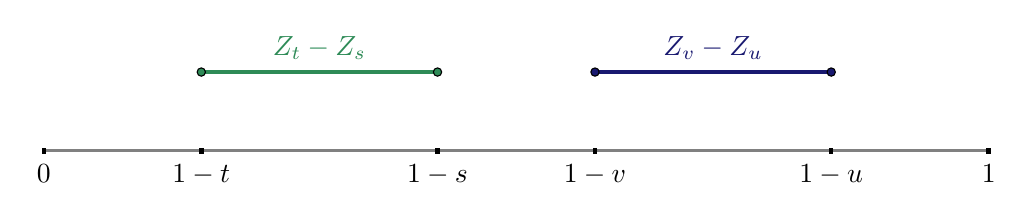
\begin{tikzpicture}
            % Main timeline
            \draw [-, very thick, color=gray] (-2,0) -- (10,0) node[below] {\(  \)};
            \foreach \x/\xtext in {-2/0, 0/1-t, 3/1-s, 5/1-v, 8/1-u, 10/1}
                \draw [ultra thick] (\x cm,1pt) -- (\x cm,-1pt) node[anchor=north] {$\xtext$};

            % # Adapted
            % f_{i-1}
            \draw [very thick, color=SeaGreen] (0,1) -- (3,1);
            \draw[color=SeaGreen] (1.5,1.3) node {\( Z_t - Z_s \)};
            \draw [fill=SeaGreen] (0,1) circle (1.5pt);
            \draw [fill=SeaGreen] (3,1) circle (1.5pt);

            % # Instantly independent

            % \phi_j
            \draw [very thick, color=MidnightBlue] (5,1) -- (8,1);
            \draw[color=MidnightBlue] (6.5,1.3) node {\( Z_v - Z_u \)};
            \draw [fill=MidnightBlue] (5,1) circle (1.5pt);
            \draw [fill=MidnightBlue] (8,1) circle (1.5pt);

            % Setup and bounding box
            % \clip(-2,-1) rectangle (9,3);
            % \draw (current bounding box.north east) rectangle (current bounding box.south west);
        \end{tikzpicture}
        \caption{The disjoint increments of \( Z \).}
        \label{fig:reverse_Wiener_increments}
    \end{figure}

    Consider the function \( θ : 𝒞 → 𝒞 : ϕ(t) ↦ ϕ(1-t) \), where \( 𝒞 \) is the space of continuous functions. Note that \( θ \) is an continuous involution on \( 𝒞 \). Moreover,
    \[ θ(\sqrt{ϵ} Z_t)  = θ(\sqrt{ϵ} (W_1 - W_{1-t})) = \sqrt{ϵ} (W_1 - W_t) = \sqrt{ϵ} V^t ∼ ν^ϵ . \]
    Using the continuity principle (\cref{thm:LDP_continuity_principle}) along with the rate function \( I \) from \cref{thm:Schilder}, \( \br{ν^ϵ}_{ϵ > 0} \) follows a large deviation principle with the rate function given by
    \begin{align*}
        J(ϕ)
        & =  I ∘ θ^{-1} (ϕ(⋅))  =  I(ϕ(1 - ⋅)) \\
        & =  \begin{cases}
            \frac12 ∫_0^1 \abs{f(t)}^2 \dif t  &  \text{if } ϕ(1 - t) = ∫_0^t f(s) \dif s \text{ for some } f ∈ L^2[0, 1]  \\
            ∞  &  \text{otherwise}
        \end{cases}  \\
        & =  \begin{cases}
            \frac12 ∫_0^1 \abs{f(t)}^2 \dif t  &  \text{if } ϕ(t) = ∫_0^{1-t} f(s) \dif s \text{ for some } f ∈ L^2[0, 1]  \\
            ∞  &  \text{otherwise} .
        \end{cases}
    \end{align*}
\end{proof}


The extension of Schilder's theorem to Itô diffusions is the content of the \emph{Freidlin–Wentzell theory}\index{Freidlin–Wentzell theory}. We start with a simple situation where we perturb an ordinary differential equation with a diffusion that goes to zero as \( ϵ → 0 \). Let \( X^ϵ \) denote the unique solution of the stochastic differential equation
\begin{equation*}
    \left\{
    \begin{aligned}
        \dif X^ϵ_t  & =  b(X^ϵ_t) \dif t + \sqrt{ϵ} \dif W_t , \\
             X^ϵ_0  & =  0 ,
    \end{aligned}
    \right.
\end{equation*}
where \( b: ℝ → ℝ \) is a uniformly Lipschitz continuous function. Let \( \br{ν^ϵ}_{ϵ > 0} \) be the sequence of probability measures induced by \( \br{X^ϵ}_{ϵ > 0} \) on \( \br{𝒞_0, \norm{⋅}_∞} \).
\begin{theorem}[{\cite[theorem 5.6.3]{DemboZeitouni1998}}]  \label{thm:LDP_Freidlin–Wentzell_simple}
    \( \br{ν^ϵ}_{ϵ > 0} \) satisfies a large deviation principle with rate function
    \begin{equation*}
        I(f) =
        \begin{cases}
            \frac12 ∫_0^1 \abs{f'(t) - b(f(t))}^2 \dif t  &  \text{if } f ∈ ℋ^1 , \\
            ∞  &  \text{otherwise} .
        \end{cases}
    \end{equation*}
\end{theorem}
The idea of the proof again rests on the continuity principle given in \cref{thm:LDP_continuity_principle}. Let us elaborate further. Suppose \( F: 𝒞_0 → 𝒞_0 \) be the deterministic map determined by \( f = F(g) \), where \( f \) is the unique continuous solution of
\[ f(t) = ∫_0^t b(f(s)) \dif s + g(t) . \]
Then \( ν^ϵ = μ^ϵ ∘ \inv{F} \), where \( μ^ϵ \) is the measure induced by \( \sqrt{ϵ} W \) on \( \br{𝒞_0, \norm{⋅}_∞} \). Now we can apply the continuity principle to arrive at the required large deviation principle result.

Finally, we look at the general case. Suppose \( κ ∈ ℝ \), the functions \( b: ℝ → ℝ \) and \( σ: ℝ → ℝ \) are bounded uniformly Lipschitz continuous functions, and \( σ \) is uniformly bounded away from \( 0 \). Let \( X^ϵ \) be the diffusion process that is the unique solution of the stochastic differential equation\index{stochastic differential equation}
\begin{equation*}
    \left\{
    \begin{aligned}
        \dif Y^ϵ_t  & =  b(Y^ϵ_t) \dif t + \sqrt{ϵ} σ(Y^ϵ_t) \dif W_t , \\
             Y^ϵ_0  & =  κ .
    \end{aligned}
    \right.
\end{equation*}
\begin{theorem}[Freidlin–Wentzell {\cite[theorem 5.6.7]{DemboZeitouni1998}}]
    The sequence of probability measures induced by \( \br{Y^ϵ}_{ϵ > 0} \) on \( \br{𝒞_0, \norm{⋅}_∞} \) satisfies a large deviation principle with rate function
    \begin{equation*}
        I_x(f) =
        \begin{cases}
            \frac12 ∫_0^1 \abs{\frac{1}{σ(f(t))} \br{f'(t) - b(f(t))}}^2 \dif t  &  \text{if } f ∈ ℋ^1_x , \\
            ∞  &  \text{otherwise} .
        \end{cases}
    \end{equation*}
\end{theorem}



\section{LSDEs with anticipating coefficients and constant initial condition}  \label{sec:LDP_constant}

In what follows, we develop a Freidlin–Wentzell type result for linear stochastic differential equations with anticipating coefficients. In particular, we look at a class of linear stochastic differential equations of the type \cref{eqn:SDE_drift} that we analyzed in \cref{chp:solving_ALSDEs}. We start off with the case of constant initial conditions.

Suppose \( σ \) and \( γ \) are deterministic functions of bounded variation on \( [0, 1] \). Moreover, suppose \( f ∈ C^2(ℝ) \) is Lipschitz continuous along with \( f, f', f'' ∈ L^1(ℝ) \). For a fixed \( κ ∈ ℝ \), consider the family of linear stochastic differential equations with parameter \( ϵ > 0 \) given by
\begin{equation}  \label{eqn:SDE_drift_LDP_constant}
    \left\{
    \begin{aligned}
        \dif Z^ϵ_κ(t)  & =  f\br{\sqrt{ϵ} ∫_0^1 γ(s) \dif W_s} Z^ϵ_κ(t) \dif t + \sqrt{ϵ} σ(t) ~ Z^ϵ_κ(t) \dif W_t  \\
             Z^ϵ_κ(0)  & =  κ ,
    \end{aligned}
    \right.
\end{equation}
Using the results from \cref{chp:solving_ALSDEs}, the unique solutions to \cref{eqn:SDE_drift_LDP_constant} are given by
\begin{align}  \label{eqn:SDE_drift_solution_Ayed–Kuo_LDP_constant}
    Z^ϵ_κ(t) =  κ \exp
    &  \left[ \sqrt{ϵ} ∫_0^t σ(s) \dif W_s - \frac{ϵ}{2} ∫_0^t σ(s)^2 \dif s \right.  \nonumber \\
    &  \left. + ∫_0^t f\br{ \sqrt{ϵ} ∫_0^1 γ(u) \dif W_u - ϵ ∫_s^t γ(u) ~ σ(u) \dif u } \dif s \right] .
\end{align}

Our approach will be similar to how the Freidlin–Wentzell results in \cref{thm:LDP_Freidlin–Wentzell_simple} are derived from Schilder's theorem (\cref{thm:Schilder}) using the continuity principle (\cref{thm:LDP_continuity_principle}). In order to use the continuity principle, we need the following lemma.

\begin{lemma}  \label{thm:θ_continuity}
    The function \( θ: 𝒞_0 → 𝒞_κ \) defined by
    \begin{align*}
        θ(x)  =  κ \exp
        &  \left[ ∫_0^t σ(s) \dif x(s) - \frac{ϵ}{2} ∫_0^t σ(s)^2 \dif s \right.  \\
        &  \left. + ∫_0^t f\br{ ∫_0^1 γ(u) \dif x(u) - ϵ ∫_s^t γ(u) ~ σ(u) \dif u } \dif s \right]
    \end{align*}
    is continuous in the topology induced by the canonical supremum norm.
\end{lemma}

\begin{proof}
    We can write
    \[ θ(x)  =  κ \exp\bs{ ϕ(x) - \frac{ϵ}{2} ∫_0^t σ_s^2 \dif s + ψ(x) } , \]
    where \( ϕ, ψ: 𝒞_0 → 𝒞_0 \) is given by
    \begin{align*}
        ϕ(x)  & =  ∫_0^t σ(s) \dif x(s)  =  σ(t) x(t) - ∫_0^t x(s) \dif σ(s) , \text{ and} \\
        ψ(x)  & =  ∫_0^t f\br{ ∫_0^1 γ(u) \dif x(u) - ϵ ∫_s^t γ(u) ~ σ(u) \dif u } \dif s .
    \end{align*}
    Using integration by parts,
    \begin{align*}
        ϕ(x)  & =  σ(t) x(t) - ∫_0^t x(s) \dif σ(s) , \text{ and} \\
        ψ(x)  & =  ∫_0^t f\br{ γ(1) x(1) - ∫_0^1 x(s) \dif γ(s) - ϵ ∫_s^t γ(u) ~ σ(u) \dif u } \dif s .
    \end{align*}
    Since multiplication by \( κ \exp\br{- \frac{ϵ}{2} ∫_0^t σ_s^2 \dif s} \) and \( \exp \) are continuous transformations, continuity of \( θ \) is guaranteed if we prove continuity of \( ϕ \) and \( ψ \). This is what we show below. For \( ϕ \), we have
    \begin{align*}
        \norm{ϕ(x) - ϕ(y)}_∞
        & =  \norm{\br{σ(t) x(t) - ∫_0^t x(s) \dif σ(s)} - \br{σ(t) y(t) - ∫_0^t y(s) \dif σ(s)}}_∞  \\
        & ≤  \norm{σ(t) \br{x(t) - y(t)}}_∞ + \norm{∫_0^t (x(s) - y(s)) \dif σ(s)}_∞  \\
        & ≤  \norm{σ}_∞ \norm{x - y}_∞  +  \abs{σ(t) - σ(0)} \norm{x - y}_∞  \\
        & ≤  3 \norm{σ}_∞ \norm{x - y}_∞ ,
    \end{align*}
    so \( ϕ \) is continuous.

    For \( ψ \), if \( L_f \) is the Lipschitz constant for \( f \), we get
    \begin{align*}
        \norm{ψ(x) - ψ(y)}_∞
        ≤ &  \left\lVert ∫_0^t L_f \left[ \br{ γ(1) x(1) - ∫_0^1 x(s) \dif γ(s) - \cancel{ϵ ∫_s^t γ(u) ~ σ_u \dif u} } \right. \right.  \\
        & \qquad  - \left. \left. \br{ γ(1) y(1) - ∫_0^1 y(s) \dif γ(s) - \cancel{ϵ ∫_s^t γ(u) ~ σ_u \dif u} } \right] \dif s \right\rVert_∞  \\
        ≤ &  L_f \norm{ ∫_0^t \br{γ(1) \br{x(1) - y(1)} - ∫_0^1 \br{x(s) - y(s)} \dif γ(s)} \dif s }_∞  \\
        ≤ &  L_f \br{\norm{γ}_∞ \norm{x - y}_∞ + \abs{γ(1) - γ(0)} \norm{x - y}}_∞  \\
        = &  3 L_f \norm{γ}_∞ \norm{x - y}_∞ ,
    \end{align*}
    which proves the continuity of \( ψ \).
\end{proof}


The following result now follows directly from the continuity of \( θ \) (\cref{thm:θ_continuity}), the continuity principle (\cref{thm:LDP_continuity_principle}), and Schilder's theorem (\cref{thm:Schilder}).
\begin{theorem}  \label{thm:SDE_drift_LDP_constant}
    The laws of the solutions \( Z^ϵ_κ \) given by \cref{eqn:SDE_drift_solution_Ayed–Kuo_LDP_constant} of the family of stochastic differential equations given by \cref{eqn:SDE_drift_LDP_constant} follow a large deviation principle on \( \br{𝒞_κ, \norm{⋅}_∞} \) with the rate function
    \begin{equation}  \label{eqn:SDE_drift_LDP_rate}
        J(y) = \inf \bc{I ∘ \inv{θ} (y)} ,
    \end{equation}
    where \( θ \) is as defined in \cref{thm:θ_continuity}, and \( I \) is the Schilder's rate function given in \cref{thm:Schilder}.
\end{theorem}



\section{LSDEs with anticipating coefficients and random initial condition}  \label{sec:LDP_random}

Is it not necessary for the family of linear stochastic differential equations \cref{eqn:SDE_drift_LDP_constant} to start at a constant point \( κ ∈ ℝ \) in order for it to have a large deviation principle. In this section, we generalize \cref{thm:SDE_drift_LDP_constant} and show that we can derive a similar result under a stronger version of exponential equivalence\index{exponential equivalence} and more restrictive conditions on the functions \( f \), \( σ \), and \( γ \).

Suppose \( σ \) and \( γ \) are deterministic functions of bounded variation on \( [0, 1] \). Moreover, suppose \( f ∈ C^2(ℝ) \) is Lipschitz continuous along with \( f, f', f'' ∈ L^1(ℝ) \). Consider the family of linear stochastic differential equations with parameter \( ϵ > 0 \) given by
\begin{equation}  \label{eqn:SDE_drift_LDP_random}
    \left\{
    \begin{aligned}
        \dif Z^ϵ_ξ(t)  & =  f\br{\sqrt{ϵ} ∫_0^1 γ(s) \dif W_s} Z^ϵ_ξ(t) \dif t + \sqrt{ϵ} σ_t ~ Z^ϵ_ξ(t) \dif W_t  \\
             Z^ϵ_ξ(0)  & =  ξ^ϵ ,
    \end{aligned}
    \right.
\end{equation}
where \( ξ^ϵ \)s are random variables independent of the Wiener process \( W \). Just as before, the unique solutions to \cref{eqn:SDE_drift_LDP_random} are given by
\begin{align}  \label{eqn:SDE_drift_solution_Ayed–Kuo_LDP_random}
    Z^ϵ_ξ(t) =  ξ^ϵ \exp
    &  \left[ \sqrt{ϵ} ∫_0^t σ(s) \dif W_s - \frac{ϵ}{2} ∫_0^t σ(s)^2 \dif s \right.  \nonumber \\
    &  \left. + ∫_0^t f\br{ \sqrt{ϵ} ∫_0^1 γ(u) \dif W_u - ϵ ∫_s^t γ(u) ~ σ(u) \dif u } \dif s \right]
\end{align}

We now state a more general large deviation principle.
\begin{theorem}
    Let \( κ ∈ ℝ \) and consider the family of random variables \( ξ^ϵ \) such that the following hold
    \begin{equation}  \label{eqn:SDE_drift_LDP_exponential_equivalence}
        \lim_{ϵ → 0} ϵ \log \E\bs{\br{ξ^ϵ - κ}^2} = -∞ .
    \end{equation}
    Moreover, assume that the functions \( f, f', σ, γ \) are all bounded. Then the laws of the solutions \( Z^ϵ_ξ \) given by \cref{eqn:SDE_drift_solution_Ayed–Kuo_LDP_random} of the family of stochastic differential equations given by \cref{eqn:SDE_drift_LDP_random} follow a large deviation principle on \( \br{𝒞_κ, \norm{⋅}_∞} \) with the rate function given by \cref{eqn:SDE_drift_LDP_rate}, where \( θ \) is as defined in \cref{thm:θ_continuity}, and \( I \) is the Schilder's rate function given in \cref{thm:Schilder}.
\end{theorem}
\begin{proof}
    Let \( V^ϵ = Z^ϵ_ξ - Z^ϵ_κ \). Then \( V^ϵ \) satisfies the stochastic differential equation
    \begin{equation}  \label{eqn:SDE_drift_LDP_difference}
        \left\{
        \begin{aligned}
            \dif V^ϵ(t)  & =  f\br{\sqrt{ϵ} ∫_0^1 γ(s) \dif W_s} V^ϵ(t) \dif t + \sqrt{ϵ} σ_t V^ϵ(t) \dif W_t  \\
                 V^ϵ(0)  & =  ξ^ϵ - κ ,
        \end{aligned}
        \right.
    \end{equation}
    whose solution is given by
    \begin{align*}
        V^ϵ(t)  =  \br{ξ^ϵ - κ} \exp
        &  \left[ \sqrt{ϵ} ∫_0^t σ_s \dif W_s - \frac{ϵ}{2} ∫_0^t σ_s^2 \dif s \right.  \\
        &  \left. + ∫_0^t f\br{ \sqrt{ϵ} ∫_0^1 γ(u) \dif W_u - ϵ ∫_s^t γ(u) ~ σ_u \dif u } \dif s \right] .
    \end{align*}

    Let \( ϕ(z) = \abs{z}^2 \) and let \( U^ϵ = ϕ(V^ϵ) \). From \cref{thm:SDE_drift_solution_squared}, \( U^ϵ \) satisfies the integral equation
    \begin{align*}
        U^ϵ(t)  =
        &  \br{ξ^ϵ - κ}^2  +  2 \sqrt{ϵ} ∫_0^t σ_s ~ U^ϵ(s) \dif W_s  \\
        & +  ϵ ∫_0^t σ_s^2 ~ U^ϵ(s) \dif s  +  f\br{∫_0^1 \sqrt{ϵ} ~ γ(s) \dif W_s} ∫_0^t U^ϵ(s) \dif s  \\
        & +  2 ϵ ∫_0^t γ(s) ~ σ_s ~ U^ϵ(s) ∫_0^s f'\br{∫_0^1 \sqrt{ϵ} ~ γ(v) \dif W_v - ϵ ∫_u^s γ(v) ~ σ_v \dif v} \dif u \dif s .
    \end{align*}

    Fix \( δ > 0 \) and let \( τ = \inf\bc{t ∈ [0, 1] : \abs{V^ϵ(t)} ≥ δ} \). Taking expectation of the stopped process \( U^ϵ(t ∧ τ) \), we get
    \begin{align*}
        &  \E\br{U^ϵ(t ∧ τ)}  \\
        & =  \E\bs{\br{ξ^ϵ - κ}^2}  +  2 \sqrt{ϵ} \E\bs{∫_0^{t ∧ τ} σ_s ~ U^ϵ(s ∧ τ) \dif W_s}  \\
        & \quad +  ϵ \E\bs{∫_0^{t ∧ τ} σ_s^2 ~ U^ϵ(s ∧ τ) \dif s}  +  \E\bs{f\br{∫_0^1 \sqrt{ϵ} ~ γ(s) \dif W_s} ∫_0^{t ∧ τ} U^ϵ(s ∧ τ) \dif s}  \\
        & \quad +  2 ϵ \E\bs{∫_0^{t ∧ τ} γ(s) ~ σ_s ~ U^ϵ(s ∧ τ) ∫_0^s f'\br{∫_0^1 \sqrt{ϵ} ~ γ(v) \dif W_v - ϵ ∫_u^s γ(v) ~ σ_v \dif v} \dif u \dif s} .
    \end{align*}
    The second integral on the right-hand side is a near-martingales by \cref{thm:Ayed–Kuo_integral_near-martingale}. Suppose \( f, f', σ, γ \) are all bounded by some \( M > 1 \). Using non-negativity of \( U^ϵ \) and the near-martingale optional stopping theorem (\cref{thm:optional_stopping_near-martingale_special}), we get
    \begin{align*}
        \E\br{U^ϵ(t ∧ τ)}
        ≤ &  \E\bs{\br{ξ^ϵ - κ}^2}  +  0  \\
          & +  ϵ M^2 \E\bs{∫_0^{t ∧ τ} U^ϵ(s ∧ τ) \dif s}  +  M \E\bs{∫_0^{t ∧ τ} U^ϵ(s ∧ τ) \dif s}  \\
          & +  2 ϵ M^3 \E\bs{∫_0^{t ∧ τ} U^ϵ(s ∧ τ) \dif s}  \\
        ≤ &  \E\bs{\br{ξ^ϵ - κ}^2} + \br{M + 2 ϵ M^3} \E\bs{∫_0^{t ∧ τ} U^ϵ(s ∧ τ) \dif s} .
    \end{align*}
    By Gronwall's inequality, we get
    \[ \E\br{U^ϵ(τ)}  =  \E\br{U^ϵ(1 ∧ τ)}  ≤  \E\bs{\br{ξ^ϵ - κ}^2} e^{M + 2 ϵ M^3} . \]

    Since \( ϕ(z) \) is a monotonically increasing nonnegative function in \( \abs{z} \), we use Markov's inequality to get
    \begin{equation*}
        \Pr\bc{\abs{V^ϵ(τ)} ≥ δ}
        = \Pr\bc{ϕ(V^ϵ(τ)) ≥ ϕ(δ)}
        ≤  \frac{\E\br{ϕ(V^ϵ(τ))}}{ϕ(δ)}
        =  \frac{\E\br{U^ϵ(τ)}}{δ^2}
        ≤  \frac{\E\bs{\br{ξ^ϵ - κ}^2}}{δ^2} e^{M + 2 ϵ M^3} .
    \end{equation*}
    Taking \( \log \) and multiplying by \( ϵ \), we get
    \[ ϵ \log \Pr\bc{\abs{V^ϵ(τ)} ≥ δ}  ≤  ϵ \log \E\bs{\br{ξ^ϵ - κ}^2} - 2 ϵ \log δ + ϵ (M + 2 ϵ M^3) . \]
    Finally, taking limit of \( ϵ → 0 \) and using \cref{eqn:SDE_drift_LDP_exponential_equivalence},
    \[ \lim_{ϵ → 0} ϵ \log \Pr\bc{\abs{V^ϵ(τ)} ≥ δ}  =  -∞ . \]
    This result allows us to say that \( Z^ϵ_ξ \) and \( Z^ϵ_κ \) are exponentially equivalent. Since exponentially equivalent families have the same large deviation principle due to \cref{thm:LDP_exponential_equivalence}, \( Z^ϵ_ξ \) follows a large deviation principle with the same rate function given by \cref{eqn:SDE_drift_LDP_rate}.
\end{proof}
